
Hoy en día es sencillo para cualquier persona con la suficiente motivación aprender a programar. De hecho, para programar en \textit{JavaScript} (ECMAScript) utilizando un entorno de ejecución como \textit{NodeJS} sobre un framework como \textit{React}, ni siquiera necesitas conocimientos sobre \textit{hardware}, ni saber como se gestiona la memoria, ni hasta cierto punto la naturaleza de un "puntero". Sin embargo, podríamos decir que estarías "programando". Creo que cada vez es más accesible y tenemos más herramientas para poder plasmar nuestras ideas a través de la propia programación, y a la vez tanta abstracción nos aleja de la cantidad de pasos que hay detrás de cada línea de código.\\\\
La primera vez que intente programar tenía trece años, e intente aprender \textit{Java} mediante unos tutoriales de \textit{Youtube}. En uno de los primeros vídeos, explicaba como se compila el código y las fases que atraviesa hasta convertirse en código máquina. Allí, lo explicaban de manera muy sencilla, primero tienes el código fuente, ese código se transforma en \textit{bytecode} (o código intermedio), y ese \textit{bytecode} pasa por una máquina virtual (JVM, Java Virtual Machine) para convertirse en código máquina. Resulta que el proceso de compilación me llamó la atención, y es por esto que he escrito mi propio ``mini''  lenguaje, al que he llamado GoneFSR, siguiendo las instrucciones y la estructura que propone David Beazley en su curso. (estos dos parrafos tal vez haya que pasarlos a la introduccion)\\\\
El compilador está basado en el curso de David Beazley, en el que explica como desarrollado un compilador llamado \textit{BeGone}, sin embargo debido a algunas extensiones de este compilador que se han realizado además de la completa implementación de las funcionalidadas requeridas por el curso, he decidido llamarlo GoneFSR. \\\\
En las siguientes subsecciones analizaremos cada parte que componen este compilador frontend. Cuando compilas código en GoneFSR, el compilador pasa por varias etapas: análisis sintáctico, análisis semántico, análisis de errores, generación de código intermedio y generación de código llvm (Low Level Virtual Machine). Ese código llvm será traducido a un ejecutable por CLANG, como último paso. A continuación veremos que significa todo esto, además de algunos detalles sobre la implementación de cada etapa.
\newpage
\section{Análisis léxico}
En un idioma cualquiera,  el léxico se entiende como el conjunto de palabras y expresiones que pertenecen a esa lengua. Al módulo del compilador, encargado del análisis léxico o tokenizado se le suele llamar \textit{Lexer}. Y su función, es por consiguiente asegurarse de que todas las palabras del archivo de entrada, pertenecen al lenguaje de programación. \\\\
Para poder llevar a cabo este proceso, el \textit{Lexer} divide la cadena de caracteres de entrada (contenido del archivo ``.g``)en \textit{tokens}. Para encontrar cada token recorre la cadena implementando un autómata finito que transiciona de estado en función del carácter que está recorriendo pasa de un estado a otro y acaba devolviendo los tipos de tokens que hemos definido en la clase como expresiones regulares. El orden en el que se definen los tokens tiene importancia, definir un token antes que otro en los que los dos comparten el comienzo del patrón, significa que se le dará prioridad al definido previamente, es por esto que todos los tokens del lenguaje se definen antes que los identificadores, ya que la REGEX de los identificadores engloba a palabras clave, como ``bool`` o ``char``. (grafismo lexer como en tfg Eduardo)
\\\\
Por \textit{token} se entienden todo tipo de palabra tanto clave como identificador, así como delimitadores como los paréntesis o el punto y coma. Aunque la función principal del \textit{Lexer} es generar tokens, también se encarga de ignorar algunos caracteres que no necesitamos que se traten como \textit{tokens} para que estos no pasen a la segunda fase, que sería el \textit{parsing} o análisis semántico, un buen ejemplo de esto son los caracteres de salto de línea, o los comentarios.\\\\
En GoneFSR, hay cuatro tipos distintos de datos. 
\begin{itemize}
    \item{Números enteros (int) de 32bits}
    \item{números decimales (float), este tipo de dato normalmente se asocia a números de coma flotante 32 bits, pero en este lenguaje en la fase final de compilación se mapean a double (64 bits) en las instrucciones llvm}
    \item{carácter (char)  es simplemente un único carácter estando permitidos cualquier letra o número, además de caracteres especiales como \textbackslash, \textbackslash n, \textbackslash ", \textbackslash xhh (siendo hh cualquier valor hexadecimal lo que permite representar cualquier carácter ASCII).}
    \item{cadenas de carácteres (strings) se especifican con la sintaxis ``texto`` y es importante decir que no se puede iterar sobre ellas. }\\
\end{itemize}
Todos las sentencias en GoneFSR, deben acabar en ";", como por ejemplo en lenguajes como C, o Java. En este lenguaje existen variables mutables e inmutables, para las inmutables o constantes no es necesario especificar un tipo de dato ya que se infiere del propio dato. La sintaxis para constantes sería
\begin{lstlisting}[style=goneStyle]
const ID = value;
\end{lstlisting}
En el caso de las variables mutables si se requiere que el usuario especifique un tipo de dato en concreto de los cuatro disponibles. La sintaxis sería
\begin{lstlisting}[style=goneStyle]
var ID datatype = value;
\end{lstlisting}
Las operaciones binarias disponibles en el compilador tanto para enteros como para decimales son: suma, resta, multiplicación y división. Siguiendo el estándar cada una de ellos se asocia con los símbolos +, -, *, /, respectivamente.\\\\
El compilador cuenta con las siguientes operaciones condicionales para después con las sentencias condicionales (``conditional statements``) poder  bifurcar el código, menor que ($<$), mayor que ($>$), menor o igual que ($\leq$), mayor o igual que ($\geq$), igual que (==) y no igual que (!=), todas estos operadores funcionan tanto para int como para float, pero no se pueden comparar entre tipos, siempre tienen que ser comparaciones entre el mismo tipo, ya que en este lenguaje no están implementados los \textit{castings} a otros tipos. Las comparaciones entre booleanos son las siguientes: igual que (==), no igual que (!=), ``y`` ($\And\And$) y ``o`` ($||$).\\\\
El símbolo + y -, también actúan como operadores unarios para int y float, para especificar cuando un número es positivo o negativo. Para lo booleanos existe el operador unario !, el cual sirve para negar el valor de la variables booleana. \\\\
\newpage
\noindent La primera sentencia condicional es el clásico "if", el cual cuenta con una sintaxis ampliamente extendida entre otros lenguajes.

\begin{lstlisting}[style=goneStyle]
if (condition) {
    statements
}
\end{lstlisting}

\noindent Para escribir un "if else".

\begin{lstlisting}[style=goneStyle]
if (condition) {
    statements
}
else {
    statements
}
\end{lstlisting}

\noindent En caso de querer escribir un bucle, GoneFSR, tan solo cuenta con el bucle ``while`` por simplicidad, que se escribiría con la sintaxis.

\begin{lstlisting}[style=goneStyle]
while (condition) {
    statements
}
\end{lstlisting}

\noindent Ya solo nos queda por ver como se declaran las funciones. En GoneFSR las funciones se escriben tal que así.
\begin{lstlisting}[style=goneStyle]
func function_name (*arguments) return_datatype {
    statements
}
\end{lstlisting}
Las funciones en GoneFSR siempre tienen que retornar un tipo de dato, ya que no existe el tipo de dato void como en C. Todos los flujos de cualquier función escrita deben retornar algo, si no el \textit{checker} lo evaluará como un error, el mecanismo para lograr esto es bastante interesante, en la sección análisis de errores, veremos como está implementado en detalle. Todo código que este escrito fuera de una función, se considera \textit{global}, aún no lo había mencionado pero en GoneFSR sí esta implementado un \textit{scope} propio para cada función así que cada una tiene su propio espacio para las variables. A nivel interno, por como está construido el compilador valore que la mejor opción era agrupar todo el código escrito fuera de una función y escribirlo en una función llamada ``\textit{premain}``, para luego en la función \textit{main} escribir como primera instrucción la llamada a esta función \textit{premain}.



En GoneFSR, hay dos funciones ``built-in``, es decir las puedes llamar sin necesidad de importar nada, ``print`` y ``filetonlfsr``. Desgraciadamente GoneFSR, no cuenta con implementaciones de gestor de módulos, ni \textit{garbage collection}, ni control de importaciones circular, ya que al fin y al cabo, no deja de ser un compilador con un propósito educativo.\\\\
\newpage
\noindent ¿Pero, cómo se distingue cada token, cómo se distingue un ``if`` de un  ``print``?, pues bien, en este caso haremos uso de la librería o mejor dicho, módulo de Python llamado SLY (Sly Lex Yacc). Esta librería que a su vez de dos herramientas muy conocidas llamadas lex y yacc (Yet Another Compiler Compiler), nos facilita el desarrollo de tanto lexers como parsers para el desarrollo de compiladores. Concretamente, nos facilita dos clases  \textit{Lexer} y \textit{Parser}, que nos harán más amigable el proceso de parsing y tokenizado del código fuente de nuestro lenguaje. \\\\
Pero, para abstraernos del código, explicaré lo esencial de la implementación del \textit{Lexer}. La clave está en las expresiones regulares, más conocidas como REGEX, estas nos permitirán buscar patrones y encontrar los tokens que queremos.\\\\
Dominar las expresiones regulares es complejo, hay muchas reglas que debes conoces, muchas caracteres que dependiendo del contexto significan una cosa u otra: grupos de captura, contenedores, ``lookahead`` con condiciones, caracteres comodín, etc... \\\\
Describir el funcionamiento de estos, me llevaría probablemente otras diez páginas así que consideraré que con decir que es a través de estas expresiones regulares como capturamos los \textit{tokens}, es suficiente. Para que no queden sin explicar, pondré un ejemplo, cómo distinguimos los enteros.
\begin{lstlisting}[style=pythonStyle]
INTEGER = r'0x[a-f0-9]+|0o[0-7]+|0b[10]+|d+'
\end{lstlisting}
\noindent Para aquellos entendidos en expresiones regulares, sabrán que hay un detalle que me he saltado sobre los enteros. Y es que un entero puede escribirse sobre diferentes bases, se puede escribir, en base diez, en base dos (binario), en base ocho (octal) y en base dieciséis (hexadecimal). En la expresión regular se puede distinguir que se define como un entero la cadena '0x' seguida de al menos un (símbolo +) carácter 'a', 'b', 'c', 'd', 'e' y 'f' o de un dígito del cero hasta el nueve. Con esta configuración no se aceptaran como caracteres hexadecimales aquellos escritos con letras mayúscula, esto es una decisión arbitraria, ya que sería fácil admitirlos. Con el carácter '$|$' especificamos un 'or' en la expresión es decir que también pueden admitirse escritos en octal (comenzando con '0o' y seguidos de al menos un dígito del cero al siete), escritos en binario (comenzando con '0b' y seguidos de al menos un dígito del cero al uno), o escritos en decimal que es lo que quiere decir la subcadena 'd+', es decir al menos un dígito del cero al nueve. \\\\
Para cada uno de los \textit{tokens} del lenguaje hay una expresión regular que lo describe, para consultar todas las expresiones regulares, tenéis el código original en \href{https://github.com/domingoUnican/TFGPedroCastro/blob/main/code/compilerGoneFSR/gone/tokenizer.py}{tokenizer.pyº}.



\newpage
\section{Análisis semántico}
Un \textit{token} no es nada por si solo, lo que lo define es como se relaciona con los otros \textit{tokens}. La definición de las relaciones entre tokens se le llama gramática. Y es en el \textit{Parser} donde hay que establecer las reglas de esta gramática. Estas reglas serán las que le den forma al AST (Abstract Syntax Tree) de cada programa de nuestro lenguaje, más tarde explicaremos qué es y pondremos un ejemplo de un AST.\\\\
Nos basaremos en la notación BNF (Backus Naur Formalism) para definir nuestra gramática libre de contexto, esta es la parte más importante, pues si todas las reglas están bien escritas pasarlo al \textit{Parser} será sencillo. Sin embargo, en este paso es fácil quedarse atascado pues hay que ser meticuloso con cada regla que escribes, ya que si no defines una buena estructura para el AST, los siguientes pasos pueden hacerse sumamente tediosos. \\\\
En el apéndice podéis consultar las reglas de la gramática. No entraré en detalles de la implementación porque no me parece relevante, pues si entiendes la gramática, entender la estructura de la clase \textit{Parser} es sencillo. Debo mencionar que esta sección del compilador realmente son dos clases en el proyecto, evidentemente, una de ellas es la clase \textit{Parser} que hereda directamente de la clase \textit{Parser} de SLY, pero la otra clase, es la clase encargada de definir las clases de cada nodo del AST. Hay muchas maneras de definir estos nodos, pero lo importante es que quede muy claro que nodos pueden estar asociados a su vez con otros nodos. Por ejemplo el nodo "ConstDeclaration" tiene como atributos un nombre de tipo "string" y un valor de tipo "Expression", o el nodo "BinOp" (Binary Operation) que tiene como atributos el tipo de operación, el operando izquierdo y el operando derecho.\\\\ 
Todo esto se entiende mucho mejor con un ejemplo de un AST de un programa en GoneFSR. Es un ejemplo muy sencillo, pero la idea creo que puede quedar clara con esto. Este sería el código fuente.

\begin{lstlisting}[style=goneStyle]
func main () int {
    var b int = 1;
    if 1 < 3 {
        b = 7;
        print b;
    }
    return 0;
}
\end{lstlisting}


\newpage Y este el AST asociado generado por el compilador en base a ese código.
\begin{figure}[h]
    \centering
    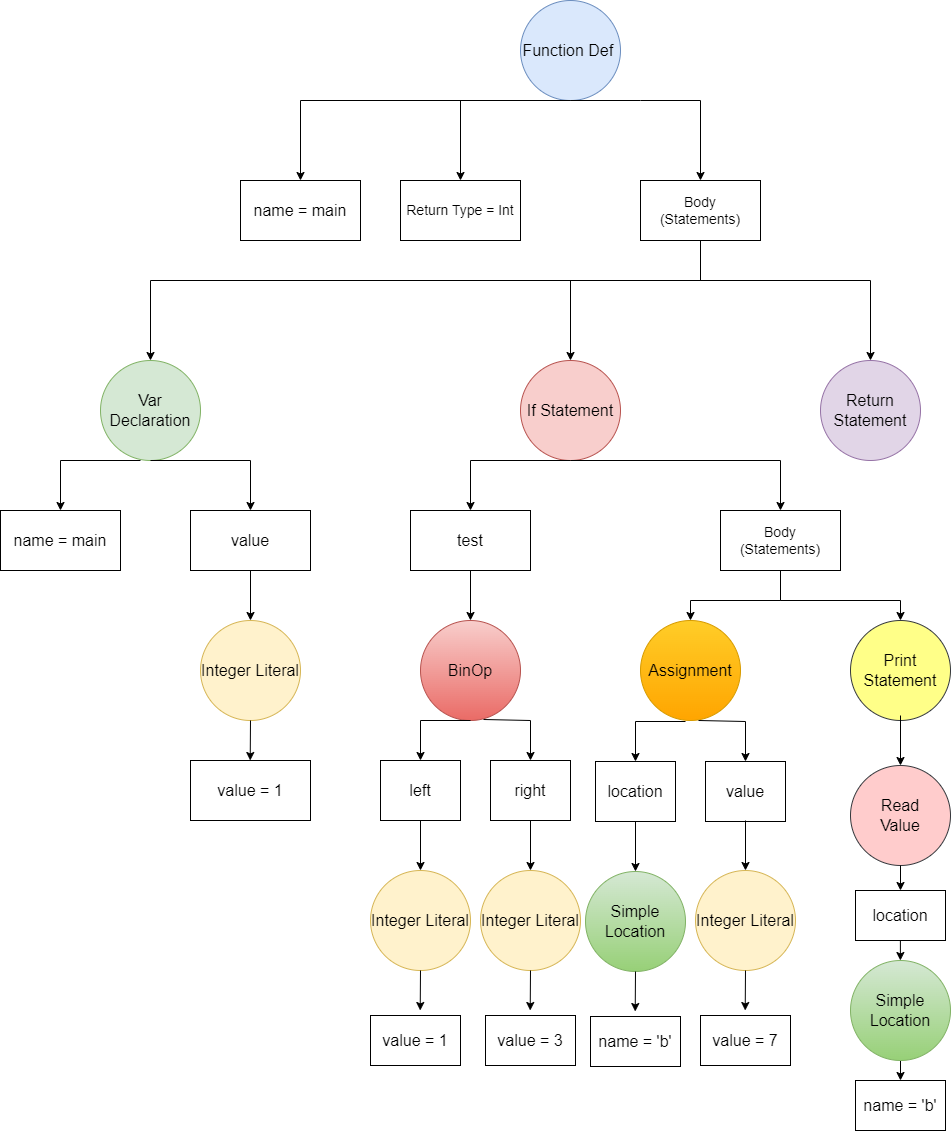
\includegraphics[width=0.9\textwidth,keepaspectratio]{img/asttree_latexexample.png} 
    \parbox{\linewidth}{\centering Ejemplo AST}
    \label{fig:mi_imagen}
\end{figure}

\newpage
(queda hablar sobre la precedencia)El AST es importante porque en los siguientes pasos lo que haremos será recorrer recursivamente este árbol para analizar errores y finalmente, generar el código intermedio. El código del \textit{Parser} se encuentra en \href{https://github.com/domingoUnican/TFGPedroCastro/blob/main/code/compilerGoneFSR/gone/parser.py}{parser.py}.
\section{Análisis de errores}
Analizar errores es un proceso complicado de programar, hay muchas cosas que pueden fallar en tiempo de ejecución y un buen compilador debe dar feedback al programador de las cosas que debe corregir para que su programa, al menos compile. Porque eso es en esencia, a lo que se dedica esta sección, a asegurarse de que todo el código fuente tiene sentido semántico, y si no lo tiene, corta el flujo del programa y no lo deja pasar a la generación de código intermedio.  \\\\
En esta fase, el compilador GoneFSR, se asegura de que todos los identificadores estén definidos antes de que se les haga referencia. Avisa de todos aquellos errores de tipado como por ejemplo asignar un valor de tipo char a una variable de tipo int. Se asegura de que las comparaciones se hacen entre valores o variables del mismo tipo de dato. Notifica si se intenta cambiar el valor de una variable cuando se trata de una constante. Revisa que no llames a una variable con el nombre de un tipo de dato, ya que estas son palabras reservadas. Todo esto, entre muchos más "\textit{checks}" que se pueden consultar en el fichero \href{https://github.com/domingoUnican/TFGPedroCastro/blob/main/code/compilerGoneFSR/gone/checker.py}{checker.py}.
\\\\
En cuanto a como se recorre el árbol, es sencillo, por cada nodo se define un método y si un nodo tiene hijos llamas al método de los hijos hasta recorrer el árbol completo y asegurarte de que no contiene errores.\\\\
Lo último que me gustaría destacar sobre este apartado es el sistema para controlar que todos los flujos de una función retornen, y en caso de que alguno de ellos no retorne lanzar un error / excepción. En una función se pueden dar dos casos, el primer caso es que la función cuente con un \textit{return} incondicional al final de la misma, por lo que el fallo estaría solventado. Y el segundo caso, en el que la función no cuenta con un return al final de la misma, por lo que hay que verificar que cada uno de los flujos de la función terminan con el \textit{return} correspondiente. ¿Cómo podemos asegurarnos de que todos los flujos terminan? \\\\ 
En GoneFSR, el problema esta solucionado de la siguiente manera. Primero recorres uno a uno los statements del \textit{body} de la función y en caso de que haya un return, lo guardas como verdadero en una variable booleana; en caso de que no haya un return en el "main flow" de la función, ocurrirá lo siguiente, durante el recorrido de cada statement de la función cada vez que se ha pasado por una bifurcación del flujo ya sea un if, un if else o un while, se ha añadido un true o un false en una lista global. Al terminar de recorrer la función, te aseguras de que todos los booleanos de esa lista sean verdaderos, en caso contrario si ademas no se ha encontrado un ``return`` en el flujo principal salta el error. Último apunte, cada vez que se visita el nodo de una función evidentemente se vacía la lista global de booleanos.
\section{Generación de código intermedio}
En Python con el módulo \textit{dis} puedes conseguir el código intermedio de cualquier bloque de código. Estudiando este código puedes conseguir un entendimiento de como funciona realmente Python, entendiendo cosas como que Python debe evaluar un símbolo cada vez que se hace uso de este. La diferencia entre entender esos de detalles y no entenderlos, es la diferencia entre un buen programador y un mal programador, ya que estas cosas suelen tener un impacto significativo en el rendimiento de un programa. Este código intermedio tiene muchas similitudes y en ocasiones durante el desarrollo de esta parte del proyecto, me he fijado en que pasaría en Python en algunos casos en concretos para luego hacer lo mismo en mi compilador. \\\\
\noindent En este paso se suelen hacer cambios para que el código funcione en cualquier máquina. Un buen ejemplo es que a pesar de que en GoneFSR existen los booleanos, en este paso los booleanos se convierten en enteros ya que hay máquinas que pueden no contar con este tipo de dato. \\\\
En GoneFSR, nuestro código intermedio se parecerá al código intermedio de Python tan solo en forma, ya que nosotros trabajaremos con menos instrucciones y no haremos tantas optimización en tiempo de compilación. Además de que las instrucciones intermedias de Python (también se les llama bytecode) se interpretan directamente por la PVM (Python Virtual Machine), ya que en Python no se hace uso de llvm por cuestiones técnicas. \\\\
Para definir el código intermedio de nuestro compilador, un estilo de código intermedio llamado \textit{Single Static Assignment} (SSA). Este paradigma se define por usar cada variable una sola vez. En la práctica esto implica que cada vez que se asigna un registro, se suma uno a un contador que a su vez es el índice del siguiente registro.Una instrucción de código intermedio puede tener los siguientes posibles argumentos: registros como operandos (``R`` + número, p.ej, ``R2``), caracteres (p. ej. para distinguir entre el tipo de comparación), y por último números enteros o flotantes. Ahora veamos la estructura de nuestras instrucciones de código intermedio.
\[ 
\texttt{ mnemónico argumento1, argumento2, \dots, argumentoN } 
\]
Existen instrucciones de manejo de memoria para cargar variables (LOAD) o almacenar valores en variables (\textsc{STORE}), entre ellas existe una distinción entre este tipo de instrucciones para variables locales y globales. También están contenidas en el código intermedio las instrucciones aritméticas y de comparación para tanto enteros como decimales. Por último, hay que mencionar a las instrucciones para crear bloques o bifurcaciones en el código. En el caso de funciones ``built-int`` (``print`` y ``fileToFSR`` cuentan con su propio mnemónico como se puede ver en el código [link a el codigo]).\\\\
Este módulo creará un diccionario con una lista de instrucciones de código intermedio para cada función. Ese diccionario se le pasará al generador de código llvm que será el encargado de dar el último paso para generar el ejecutable. 
\section{Generación de código LLVM}
LLVM es un conjunto de herramientas para el desarrollo tanto de frontend como de backend de compilación. Se define como frontend del compilador, el software encargado del análisis sintáctico o \textit{scanning}, el análisis semántico y de al menos generar una representación intermedia del código (en nuestro caso, la generación de código intermedio se hace en dos etapas). Por otro lado, el backend se define como la parte que optimiza y genera el código máquina optimizando y puliendo las instrucciones para que puedan ejecutarse en ese entorno en concreto. La ventaja más evidente de separar el proceso de compilado en estas dos etapas es que en lugar de hacer un compilador personalizado para cada lenguaje y para cada arquitectura, programas un compilador frontend para cada lenguaje y después un backend para cada arquitectura. Hay algunos compiladores que realizan las dos etapas como por ejemplo \textit{gcc}.\\\\
Veamos un ejemplo básico de uso del modulo \textit{llvm} para escribir código intermedio llvm. Siendo el código de python.
\begin{lstlisting}[style=pythonStyle]
from llvmlite.ir import Module, Function, FunctionType, IntType, IRBuilder, Constant, DoubleType, GlobalVariable, VoidType
import llvmlite.binding as llvm

# Inicializacion clases llvm
mod = Module('ejemplo')
main = Function(mod, FunctionType(IntType(32), []), name="main")
block = main.append_basic_block('entry')
builder = IRBuilder(block)

# Inicializacion variable global
global_operando = GlobalVariable(mod, IntType(32), 'globalop')
global_operando.initializer = Constant(IntType(32), 10)
valor_global_operando = builder.load(global_operando)
# Inicializacion variable local
local_operando = builder.alloca(IntType(32), name="localop")
builder.store(Constant(IntType(32), 5), local_operando)
valor_local_operando = builder.load(local_operando)
# calculo de resultado
resultado = builder.add(valor_local_operando, valor_global_operando, "resultado")
builder.ret_void()
print(str(mod))
\end{lstlisting}
Y el código llvm que obtenemos una vez ejecutamos el scritp en Python es este.
\begin{lstlisting}[style=pythonStyle]
; ModuleID = "ejemplo"
target triple = "unknown-unknown-unknown"
target datalayout = ""

define i32 @"main"()
{
entry:
  %".2" = load i32, i32* @"globalop"
  %"localop" = alloca i32
  store i32 5, i32* %"localop"
  %".4" = load i32, i32* %"localop"
  %"resultado" = add i32 %".4", %".2"
  ret void
}

@"globalop" = global i32 10
\end{lstlisting}
El código llvm es bastante ofuscado e incómodo de leer, pero es portable. Esto tiene que ver con lo mencionado anteriormente del frontend y el backend en un compilador. Ahora que tenemos el código intermedio cualquier backend ya sea llc (el backend más común para llvm), clang, o incluso el propio compilador del ``novedoso`` lenguaje Rust (la gestión de memoria de este lenguaje merecería un TFG entero).\\\\
Vamos a analizar línea a línea que está pasando en ese código llvm. Lo primero de todo, el sitio donde definimos el código se le llama módulo y se podría entender como un ``fichero``. Dentro del módulo se definen funciones, y dentro de estas funciones se definen bloques. Estos bloques parecen una cosa que está para abultar, pero nada más lejos de la realidad, son la clave a la hora de implementar sentencias condicionales, ya que nuestro código deberá saber a que bloque debe ``saltar`` (hay algunos detractores en esto de dar saltos por el código, argumentan que dar saltos en memoria puede ralentizar el tiempo de ejecución).\\\\ Ya tenemos nuestro módulo, nuestra función y nuestro bloque donde escribir código. Bien, la siguientes dos instrucciones en el script de Python inicializan una constante, si ahora nos fijamos en el código llvm, podemos ver que la constante inicializada se encuentra fuera del \textit{scope} de la función main. La siguiente línea carga el valor de la constante en una variable temporal (\%``.2``).  Después se declara una variable local como int, a esta variable se le da un valor de 5. Ahora i32 tiene un asterisco (*) detrás esto denota que actúa como puntero lo cual tiene sentido es decir estamos guardando un entero de 32 bits en la posicion de memoria de ``localop``. Cargamos el valor de ``localop`` en otra variable temporal, para luego sumar ambas variables temporales guardando la suma en una variable local con nombre "resultado". De primeras, intimida mucho más de lo que es, ya que en realidad es perfectamente legible para humanos.
\\\\
Como al generador de codigo llvm le llega el código intermedio de la etapa anterior dividido en un diccionario (o HashMap, lo llamo diccionario porque así se le llama en Python), en el que las llaves son el nombre de las funciones. Creará en el modulo llvm tantas funciones como se le pasen por parámetro en la forma de esta estructura de datos. Sabiendo esto y que este generador utiliza los bloques de las funciones para escribir los saltos condicionales creo que lo correcto es finalizar la sección con el código llvm de la función \textit{main} de la sección 2.3.
\begin{lstlisting}[style=pythonStyle]
define i32 @"main"()
{
entry:
  call void @"premain"()
  %"b" = alloca double
  store double              0x0, double* %"b"
  store double 0x3ff0000000000000, double* %"b"
  %"R2" = load double, double* %"b"
  %"R4" = fcmp olt double %"R2", 0x4008000000000000
  br i1 %"R4", label %"B1", label %"B2"
B1:
  %"R7" = fadd double 0x401c000000000000, 0x4020000000000000
  store double %"R7", double* %"b"
  %"R8" = load double, double* %"b"
  call void @"_print_float"(double %"R8")
  br label %"B2"
B2:
  ret i32 0
}
\end{lstlisting}
La llamada a \textit{premain} es porque como ya comente todo código escrito fuera de \textit{main} se ejecute en \textit{premain} en este caso no hay código fuera de \textit{main} así que la función está vacía (el código llvm es en realidad, un poco más largo). La opción de no permitir código fuera de \textit{main} era igual de válida pero yo decidí implementarlo así arbitrariamente. \\\\
Lo último que me queda por explicar es la traducción del \textit{if}, esto se hace a través de la intruccion ``br`` que si os fijáis es de tipo ``i1``, un integer de un solo bit, que es lo mismo que un booleano. Los otros dos términos de la instrucción son instrucciones label con dos etiquetas distintas ``B1`` y ``B2``. Pues bien si ese entero de un solo bit es 1 se saltará al bloque ``B1`` y en caso contrario a ``B2``. El valor de ese entero se determino en la operacion de comparación que se guarda en el registro temporal R4.

\section{Código llvm a código máquina}
CLANG actúa como backend de compilación en nuestro proyecto, ya que yo no he implementado las etapas de backend, generar el código máquina en función de la arquitectura o la etapa de enlazado. Hay que resaltar que CLANG emplea las librerías internas de LLVM para poder realizar el procecso de backend, ya que el propósito de CLANG es actuar de frontend, pero en este caso esa utilidad no nos hace falta. \\\\
En la práctica, tan solo tendremos que llamar al compilador desde la terminal y pasarle como argumentos tanto el archivo con el código intermedio llvm, como el archivo con las funciones ``built-in``. Con estos requisitos CLANG, nos escribirá un ejecutable en el directorio donde hayamos ejecutado el comando que será, en efecto nuestro programa.
\section{Implementación función fsr}

\section{Testing del compilador}


